Un microcontrolador es un sistema en un chip. Mientras que su computadora se compone de varios componentes discretos: un procesador, RAM, almacenamiento, un puerto Ethernet, etc.; un microcontrolador tiene todos esos tipos de componentes integrados en un solo ``chip'' o paquete. Esto hace posible construir sistemas con menos partes.

Los microcontroladores son la parte central de lo que se conoce como ``sistemas embebidos''. Los sistemas embebidos están en todas partes, pero normalmente no los nota. Ellos controlan las máquinas que lavan tu ropa, imprimen tus documentos y cocinan tu comida. Los sistemas embebidos mantienen los edificios en los que vive y trabaja a una temperatura agradable y controlan los componentes que hacen que los vehículos en los que viaja se detengan y arranquen.

La mayoría de los sistemas embebidos funcionan sin la intervención del usuario. Incluso si exponen una interfaz de usuario como lo hace una lavadora; la mayor parte de su operación se realiza por su cuenta.

Los sistemas embebidos se utilizan a menudo para controlar un proceso físico. Para que esto sea posible, tienen uno o más dispositivos que les informan sobre el estado del mundo (``sensores'') y uno o más dispositivos que les permiten cambiar las cosas (``actuadores''). Por ejemplo, el sistema de control climático de un edificio podría tener:

\begin{itemize}
	\item Sensores que miden la temperatura y la humedad en varios lugares.
	\item Actuadores que controlan la velocidad de los ventiladores.
	\item Actuadores que hacen que se agregue o se quite calor del edificio.
\end{itemize}

\section{¿Cuando debo usar un microcontrolador? }

Muchos de los sistemas integrados enumerados anteriormente podrían implementarse con una computadora que ejecute \textbf{Linux} (por ejemplo, una ``Raspberry Pi''). ¿Por qué usar un microcontrolador en su lugar? Parece que podría ser más difícil desarrollar un programa.

Algunas razones pueden incluir:

\begin{itemize}
	\item \textbf{Costo}. Un microcontrolador es mucho más económico que una computadora de propósito general. No solo el microcontrolador es más barato; también requiere muchos menos componentes eléctricos externos para funcionar. Esto hace que las placas de circuito impreso (\textbf{PCB}) sean más pequeñas y económicas de diseñar y fabricar.
	\item \textbf{El consumo de energía}. La mayoría de los microcontroladores consumen una fracción de la potencia de un procesador completo. Para aplicaciones que funcionan con baterías, eso marca una gran diferencia.
	\item \textbf{Sensibilidad}. Para lograr su propósito, algunos sistemas integrados siempre deben reaccionar dentro de un intervalo de tiempo limitado (por ejemplo, el sistema de frenado ``antibloqueo'' de un automóvil). Si el sistema no cumple con este tipo de fecha límite, podría ocurrir una falla catastrófica. Tal fecha límite se denomina requisito de ``tiempo real estricto''. Un sistema integrado que está sujeto a dicho plazo se denomina ``sistema duro en tiempo real''. Una computadora de uso general y un sistema operativo generalmente tienen muchos componentes de software que comparten los recursos de procesamiento de la computadora. Esto hace que sea más difícil garantizar la ejecución de un programa dentro de las estrictas limitaciones de tiempo.
	\item \textbf{Fiabilidad}. En sistemas con menos componentes (tanto de hardware como de software), ¡hay menos cosas que pueden fallar!
\end{itemize}
\section{¿Cuándo no debo usar un microcontrolador?}

Donde se involucran cálculos pesados. Para mantener bajo su consumo de energía, los microcontroladores tienen a su disposición recursos computacionales muy limitados. Por ejemplo, algunos microcontroladores ni siquiera tienen soporte de hardware para operaciones de punto flotante. En esos dispositivos, realizar una simple suma de números de precisión simple puede llevar cientos de ciclos de CPU.

\subsection{¿Por qué usar Rust y no C?}

Con suerte, no necesito convencerlo aquí, ya que probablemente esté familiarizado con las diferencias de idioma entre Rust y C. Un punto que quiero mencionar es la administración de paquetes. C carece de una solución de gestión de paquetes oficial y ampliamente aceptada, mientras que Rust tiene Cargo. Esto hace que el desarrollo sea mucho más fácil. Y, en mi opinión, la fácil administración de paquetes fomenta la reutilización del código porque las bibliotecas se pueden integrar fácilmente en una aplicación, lo que también es bueno ya que las bibliotecas obtienen más ``pruebas de batalla''.

\subsection{¿O por qué debería preferir C sobre Rust?}


El ecosistema C es mucho más maduro. Ya existe una solución lista para usar para varios problemas. Si necesita controlar un proceso sensible al tiempo, puede tomar uno de los sistemas operativos en tiempo real (RTOS) comerciales existentes y resolver su problema. Todavía no hay RTOS comerciales de grado de producción en Rust, por lo que tendría que crear uno usted mismo o probar uno de los que están en desarrollo. Puede encontrar una lista de ellos en el repositorio \textit{\textbf{Awesome Embedded Rust}}.



\section{Descripción del Hardware}

La placa STM32 Nucleo-64 proporciona una forma asequible y flexible para que los usuarios prueben nuevos conceptos y construyan prototipos eligiendo entre las diversas combinaciones de funciones de rendimiento y consumo de energía que proporciona el microcontrolador STM32. Para las placas compatibles, el \textit{SMPS} externo reduce significativamente el consumo de energía en modo Run. El soporte de conectividad ARDUINO Uno V3 y los encabezados ST morpho permiten la fácil expansión de la funcionalidad de la plataforma de desarrollo abierta STM32 Nucleo con una amplia variedad de placas de expansión especializados.

La placa STM32 Nucleo-64 no requiere ninguna sonda separada ya que integra el depurador/programador ST-LINK.

La placa STM32 Nucleo-64 viene con las completas bibliotecas de software gratuito STM32 y ejemplos disponibles con el paquete STM32Cube MCU.

\begin{figure}[htb]
	\centering
	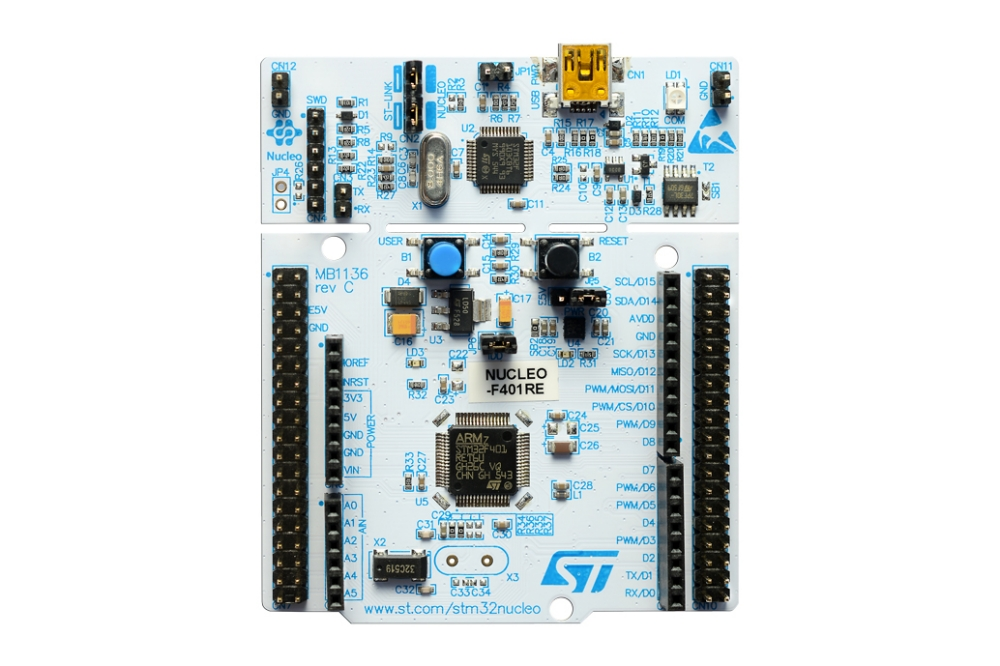
\includegraphics[width=0.7\textwidth]{capitulo1/f411re.jpg}
	\caption{Tarjeta núcleo F411RE de ST}
	\label{cap1:001}
\end{figure} 

Los dispositivos STM32F411XC/XE se basan en el núcleo RISC de 32 bits Arm® Cortex® -M4 de alto rendimiento que funciona a una frecuencia de hasta 100 MHz. El núcleo Cortex®-M4 cuenta con una unidad de punto flotante (FPU) de precisión simple que admite todas las instrucciones de procesamiento de datos y tipos de datos de precisión simple de Arm. También implementa un conjunto completo de instrucciones DSP y una unidad de protección de memoria (MPU) que mejora la seguridad de la aplicación.

El STM32F411xC/xE pertenece a la línea de productos STM32 Dynamic Efficiency™ (con productos que combinan la eficiencia energética, el rendimiento y la integración) al tiempo que agrega una nueva característica innovadora llamada Modo de adquisición por lotes (BAM) que permite ahorrar aún más el consumo de energía durante el procesamiento por lotes de datos.

El STM32F411xC/xE incorpora memorias integradas de alta velocidad (hasta 512 Kbytes de memoria Flash, 128 Kbytes de SRAM) y una amplia gama de E/S y periféricos mejorados conectados a dos buses APB, dos buses AHB y un bus de 32 bits. matriz de bus multi-AHB. Todos los dispositivos ofrecen un ADC de 12 bits, un RTC de bajo consumo, seis temporizadores de 16 bits de uso general, incluido un temporizador PWM para el control del motor, dos temporizadores de 32 bits de uso general. También cuentan con interfaces de comunicación estándar y avanzadas.

\begin{itemize}
	\item Hasta tres I2C
	\item Cinco SPI
	\item Cinco I2S de los cuales dos son full dúplex. Para lograr una precisión de clase de audio, los periféricos I2S se pueden sincronizar mediante un PLL de audio interno dedicado o mediante un reloj externo para permitir la sincronización.
	\item Tres USART
	\item Interfaz SDIO
	\item Interfaz USB 2.0 OTG de máxima velocidad
\end{itemize}


El STM32F411xC/xE opera en el rango de temperatura de - 40 a + 125 °C desde una fuente de alimentación de 1,7 (PDR OFF) a 3,6 V. Un conjunto completo de modo de ahorro de energía permite el diseño de aplicaciones de bajo consumo.

Estas características hacen que los microcontroladores STM32F411xC/xE sean adecuados para una amplia gama de aplicaciones:

\begin{itemize}
	\item Control de aplicaciones y accionamiento de motores
	\item Equipo medico
	\item Aplicaciones industriales: PLC, inversores, disyuntores
	\item Impresoras y escáneres
	\item Sistemas de alarma, video portero y climatización
	\item Electrodomésticos de audio para el hogar
	\item Concentrador de sensores de teléfonos móviles
\end{itemize}


\begin{figure}[htb]
	\centering
	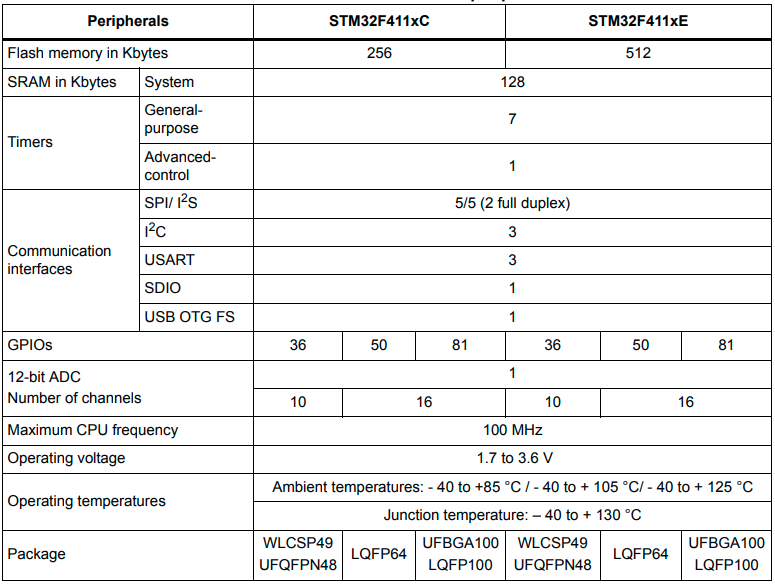
\includegraphics[width=0.9\textwidth]{capitulo1/caracteristicas.png}
	\caption{Características de la Tarjeta núcleo F411RE de ST}
	\label{cap1:002}
\end{figure} 

\subsection{Mapeo de Memoria}

El mapa de memoria de procesador es necesario para determinar la región de donde se almacenarán los códigos de los programas. En la figura \ref{cap1:003} se muestra el mapeo de memoria para este procesador.

\begin{figure}[htb]
	\centering
	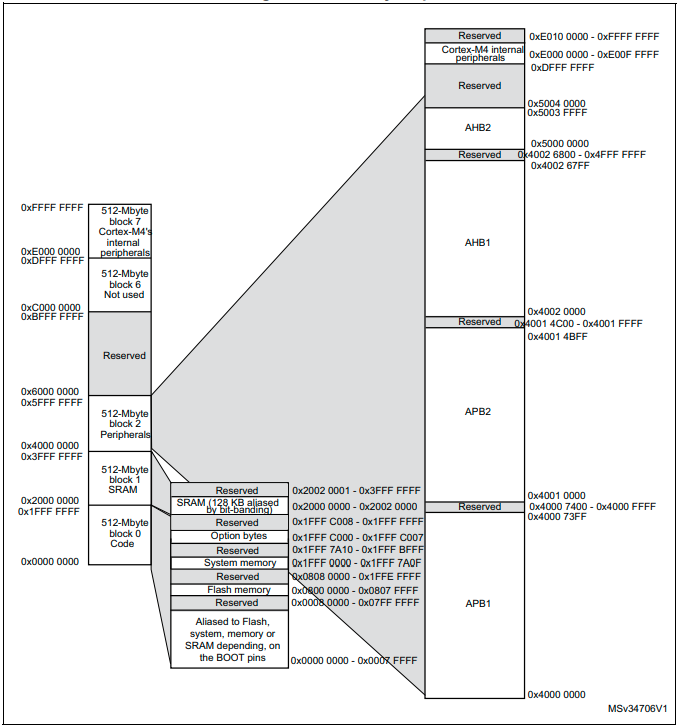
\includegraphics[width=0.9\textwidth]{capitulo1/memoria.png}
	\caption{Mapa de memoria de la Tarjeta núcleo F411RE de ST}
	\label{cap1:003}
\end{figure} 

\section{Configurando el ambiente de desarrollo}

Tratar con microcontroladores involucra varias herramientas, ya que estaremos tratando con una arquitectura diferente a la de su computadora y tendremos que ejecutar y depurar programas en un dispositivo ``remoto''.

Usaremos todas las herramientas enumeradas a continuación. Cuando no se especifica una versión mínima, cualquier versión reciente debería funcionar, pero hemos enumerado la versión que hemos probado.

\begin{itemize}
	\item \textbf{Rust} 1.53.0 o una nueva cadena de herramientas
	\item \textbf{gdb-multiarch}. Versión probada: 10.2. Sin embargo, es probable que otras versiones también funcionen. Si su distribución/plataforma no tiene gdb multiarch disponible, arm-none-eabi-gdb también funcionará. Además, algunos binarios gdb normales también están construidos con capacidades multiarquitectura, puede encontrar más información sobre esto en los subcapítulos.
	\item \textbf{cargo-binutils}. Versión 0.3.3 o más nueva.
	\item \textbf{cargo-embed}. Version 0.11.0 o más nueva.
	\item \textbf{minicom} en linux o mac. 
	\item \textbf{PuTTY} en Windows.
\end{itemize}

\subsection{Instalación de rustc y Cargo}

Rustup es un instalador para el lenguaje de programación de sistemas Rust. Ejecute lo siguiente en su terminal, luego siga las instrucciones en pantalla.


\begin{lstlisting}[language=bash]
$\$$ curl --proto '=https' --tlsv1.2 -sSf https://sh.rustup.rs | sh
\end{lstlisting} 

Después de ejecutar el comando anterior en una terminal obtenemos la respuesta que aparece en la figura \ref*{cap1:004}. 

\begin{figure}[htb]
	\centering
	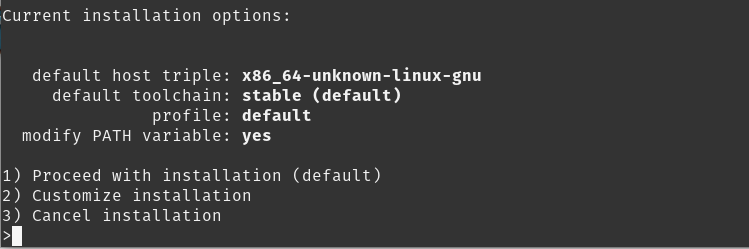
\includegraphics[width=0.9\textwidth]{capitulo1/rustup.png}
	\caption{Opciones de instalación de Rust}
	\label{cap1:004}
\end{figure} 

De la cual elegimos \textbf{la opción 1}, después de lo cual nos instala Rust y nos modifica la variable path de nuestras terminales para poder ejecutar el comando rustc y cargo. Ahora verificamos la versión de rustc y cargo que se instalaron:

\begin{lstlisting}[language=bash]
	$\$$ rustc -V
		rustc 1.57.0 (f1edd0429 2021-11-29)
	$\$$ cargo -V
		cargo 1.57.0 (b2e52d7ca 2021-10-21)	
\end{lstlisting} 

\subsection{Instalación de cargo-binutils}

\begin{lstlisting}[language=bash]
	$\$$ rustup component add llvm-tools-preview

	$\$$ cargo install cargo-binutils
		
	$\$$ cargo-size --version
\end{lstlisting} 

\subsection{cargo-embed}

\begin{lstlisting}[language=bash]
	$\$$ cargo install cargo-embed
	
	$\$$ cargo embed --version
\end{lstlisting} 

Si marca error el primer comando es porque el sistema no tiene instalado la librería \textit{libudev}

\begin{lstlisting}[language=bash]
	$\$$ sudo apt update
	$\$$ sudo apt-get install -y libudev-dev
\end{lstlisting} 

Después de instalar la librería \textbf{libudev} ya es posible instalar \textbf{cargo-embed}. 

\subsection{Instalación en linux}

Estos son los comandos de instalación para algunas distribuciones de Linux.

\begin{lstlisting}[language=bash]
	$\$$ sudo apt-get install gdb-multiarch minicom
\end{lstlisting} 

\subsubsection{reglas udev}

Para establecer las reglas udev y que linux detecte la tarjeta, \textbf{debemos primero conectar la tarjeta} y posteriormente ejecutar el siguiente comando:

 \begin{lstlisting}[language=bash]
 	$\$$ lsusb
 \end{lstlisting} 

Lo cual produce la salida que se muestra en la figura \ref{cap1:005}

\begin{figure}[htb]
	\centering
	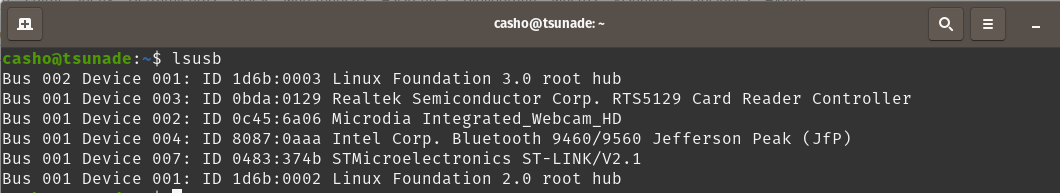
\includegraphics[width=0.9\textwidth]{capitulo1/lsusb.png}
	\caption{Salida del comando lsusb }
	\label{cap1:005}
\end{figure} 

De la figura \ref{cap1:005} podemos ver los datos

\begin{lstlisting}[language=bash]
Bus 001 Device 007: ID 0483:374b STMicroelectronics ST-LINK/V2.1
\end{lstlisting} 

De donde los datos del ID corresponden a: \textbf{idVendor:idProduct}. Que utilizaremos para la creación de las reglas udev.

Estas reglas le permiten usar dispositivos USB como ST-LINK sin privilegios de root, es decir, sudo. Cree un archivo en directorio \textbf{/etc/udev/rules.d} con el contenido que se muestra a continuación.

\begin{lstlisting}[language=bash]
$\$$ sudo nano /etc/udev/rules.d/99-stlink.rules
\end{lstlisting} 

El contenido del archivo debe ser:

\begin{lstlisting}[language=bash]
# CMSIS-DAP for stlink
SUBSYSTEM=="usb", ATTR{idVendor}=="0483", ATTR{idProduct}=="374b", MODE:="666"
\end{lstlisting} 

Luego recarga las reglas de udev con:

\begin{lstlisting}[language=bash]
$\$$ sudo udevadm control --reload-rules
\end{lstlisting} 

Si tenía alguna placa conectada a su computadora, desenchúfela y luego vuelva a enchufarla.

\section{Instalación en windows}

ARM proporciona instaladores .exe para Windows. Tome uno de aquí (\textbf{\textit{https://developer.arm.com/tools-and-software/open-source-software/developer-tools/gnu-toolchain/gnu-rm/downloads}}) y siga las instrucciones. Justo antes de que finalice el proceso de instalación, marque/seleccione la opción ``Agregar ruta a la variable de entorno''. Luego verifique que las herramientas estén en su \textbf{PATH}:

\begin{lstlisting}[language=bash]
	$\$$ arm-none-eabi-gcc -v
\end{lstlisting} 

\subsection{Instalación de PuTTY}

Descargue el último \textbf{putty.exe} de este sitio(\textbf{https://www.chiark.greenend.org.uk/~sgtatham/putty/latest.html}) y colóquelo en algún lugar de su \textbf{PATH}.

\section{Instalación de MacOs} 

Todas las herramientas se pueden instalar usando Homebrew:

\begin{lstlisting}[language=bash]
$\$$ brew tap ArmMbed/homebrew-formulae
$\$$ brew install arm-none-eabi-gcc
$\$$ brew install minicom
\end{lstlisting} 

\section{Verificando cargo-embed}

Primero, conecte la tarjeta a su computadora usando un cable USB.

\subsection{Paso 1: Cree un proyecto}

Primero creamos un nuevo proyecto:

\begin{lstlisting}[language=bash]
$\$$ cargo new ejemplo1
$\$$ cd ejemplo1
$\$$ code .
\end{lstlisting} 


A continuación, deberá crear el archivo \textbf{Embed.toml} en el directorio donde se encuentre el archivo \textbf{Cargo.toml}. En la sección \textbf{default.general} encontrará dos variantes de chips comentadas:

\begin{lstlisting}[language=bash]
# Archivo Embed.toml
[default.probe]
protocol = "Swd"

[default.general]
# chip = "nrf52833_xxAA" # uncomment this line for micro:bit V2
# chip = "nrf51822_xxAA" # uncomment this line for micro:bit V1

[default.rtt]
enabled = true

[default.gdb]
enabled = false
\end{lstlisting}

Ahora se modifica el archivo \textbf{Cargo.toml} 

\begin{lstlisting}[language=bash]
# Archivo Cargo.toml
[package]
name = "ejemplo1"
version = "0.1.0"
edition = "2021"

[dependencies]
cortex-m = "0.7.3"
cortex-m-rt = "0.7.0"
rtt-target = { version =  "0.3.1", features = ["cortex-m"] }
panic-rtt-target = { version =  "0.1.2", features = ["cortex-m"] }
\end{lstlisting}

Ahora se crea un archivo \textbf{memory.x} donde se indica la distribución de memoria, este archivo debe estar en el directorio donde se encuentre el archivo \textbf{Cargo.toml}.

\begin{lstlisting}[language=bash]
# archivo de memory.x
MEMORY
{
	/* NOTE K = KiBi = 1024 bytes */
	FLASH : ORIGIN = 0x00000000, LENGTH = 512K
	RAM : ORIGIN = 0x20000000, LENGTH = 128K
}
\end{lstlisting}

Ahora modificamos el archivo \textbf{src/main.rs} 

\begin{lstlisting}[language=c]
# archivo de src/main.rs
#![no_std]
#![no_main]

use panic_rtt_target as _;
use rtt_target::{rtt_init_print, rprintln};

use cortex_m_rt::entry;

#[entry]
fn main() -> ! {
	rtt_init_print!();
	rprintln!("Hola Mundo");
	loop {}
}

\end{lstlisting}

Ahora en el raíz creamos un directorio llamado \textbf{.cargo}, en donde dentro de este creamos el archivo \textbf{config}, con el siguiente contenido:

\begin{lstlisting}[language=bash]
[target.'cfg(all(target_arch = "arm", target_os = "none"))']
rustflags = [
"-C", "link-arg=-Tlink.x",
]
\end{lstlisting}

Ahora instalamos la compilación cruzada:

\begin{lstlisting}[language=bash]
$\$$ rustup target add thumbv7em-none-eabihf
$\$$ cargo embed --target thumbv7em-none-eabihf
\end{lstlisting}

Después de lo cual debemos observar ``Hola Mundo'' en la terminal.